\section{Methodology}
\label{sec:method}

\subsection{FFT Preprocessing}
\label{sec:fftpre}

The FFT branch converts each normalised RGB image into a
frequency-domain representation via the following six-step pipeline
(\cref{fig:fftcompare}):

\begin{enumerate}
  \item \textbf{Denormalise.}  Reverse ImageNet mean/std to recover $[0,1]$
    pixel values.
  \item \textbf{2-D DFT.}  Apply \texttt{numpy.fft.fft2} per channel.
  \item \textbf{FFT shift.}  Centre the DC component with
    \texttt{fftshift}.
  \item \textbf{Log-magnitude.}  Compute $\log(|F_{uv}| + \varepsilon)$,
    $\varepsilon\!=\!10^{-8}$.
  \item \textbf{Min–max normalise.}  Scale each channel to $[0,1]$.
  \item \textbf{Re-normalise.}  Re-apply ImageNet statistics for consistent
    ResNet18 input scale.
\end{enumerate}

The resulting $224\!\times\!224\!\times\!3$ tensor captures the 2-D spectral
energy distribution.
As shown in \cref{fig:fftcompare}, StyleGAN2 faces exhibit a characteristic
cross-hair pattern of elevated energy along the horizontal and vertical
frequency axes — a direct consequence of periodic transposed-convolution
upsampling artefacts.

\begin{figure*}[t]
  \centering
  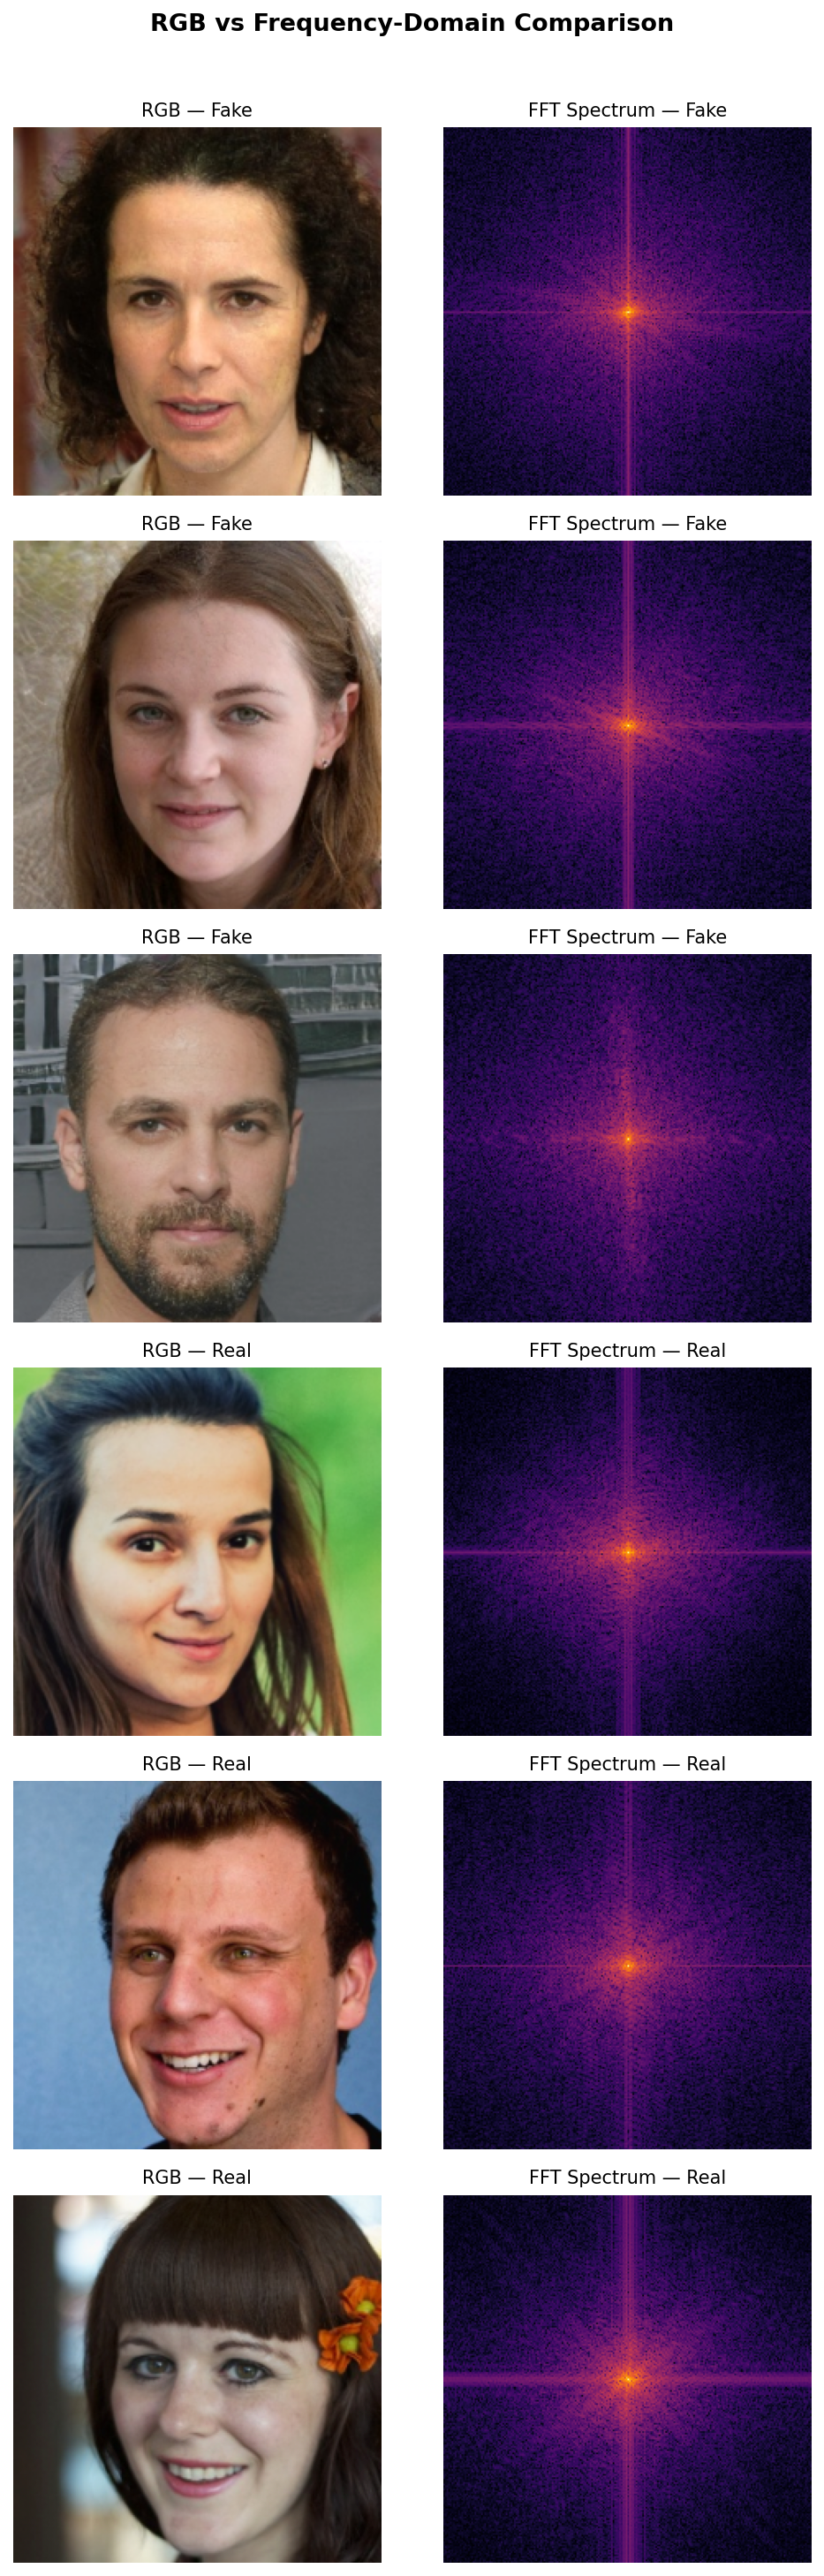
\includegraphics[width=\textwidth]{results/figures/rgb_vs_fft_comparison.png}
  \caption{%
    \textbf{RGB vs.\ FFT spectrum comparison.}
    Top row: raw face images (real left, StyleGAN2-generated right).
    Bottom row: corresponding log-magnitude FFT spectra.
    GAN-generated faces show bright horizontal/vertical streaks through the
    DC centre — periodic artefacts from transposed-convolution upsampling.
  }
  \label{fig:fftcompare}
\end{figure*}

\subsection{Model Architectures}
\label{sec:models}

All models use ResNet18~\cite{he2016resnet} as the backbone: four residual
stages followed by global average pooling to produce a 512-d feature vector.
The original ImageNet head is removed and replaced by a detection head.

\paragraph{RGB model.}
ImageNet-pretrained ResNet18 with head:
$\text{Dropout}(0.3) \to \text{Linear}(512, 2)$.

\paragraph{FFT model.}
Identically structured ResNet18 but \emph{randomly initialised} — no
ImageNet pretraining — since the FFT input distribution has no natural
correspondence to RGB images.
Same head: $\text{Dropout}(0.3) \to \text{Linear}(512, 2)$.

\paragraph{Hybrid model.}
Two independent ResNet18 branches (RGB: ImageNet-pretrained; FFT: random
init) extract 512-d feature vectors each.
The vectors are concatenated to a 1{,}024-d fused representation:
\begin{equation}
  \mathbf{z} =
    \bigl[ f_{\text{RGB}}(\mathbf{x}_{\text{rgb}})\,;
           f_{\text{FFT}}(\mathbf{x}_{\text{fft}}) \bigr]
    \in \mathbb{R}^{1024}
  \label{eq:fusion}
\end{equation}
The classification head is:
$\text{Dropout}(0.4) \to \text{FC}(1024,256) \to \text{ReLU}
 \to \text{Dropout}(0.3) \to \text{FC}(256,2)$.

\subsection{Training Configuration}
\label{sec:training}

All models minimise cross-entropy loss using Adam~\cite{kingma2015adam}
($L_2$ weight decay $10^{-4}$) with ReduceLROnPlateau
(factor\,=\,0.5, patience\,=\,2) and early stopping (patience\,=\,3 on
validation loss).
The best checkpoint (lowest val-loss epoch) is restored before evaluation.
Per-experiment hyperparameters are listed in \cref{tab:hparams}.

\begin{table}[t]
  \centering
  \caption{Per-experiment training settings.  Batch size, training images,
    and early-stopping patience are identical across all three experiments.}
  \label{tab:hparams}
  \small
  \begin{tabular}{@{}lccc@{}}
    \toprule
    \textbf{Setting} & \textbf{RGB} & \textbf{FFT} & \textbf{Hybrid} \\
    \midrule
    Learning rate & $10^{-4}$ & $10^{-3}$ & $5\!\times\!10^{-5}$ \\
    Pretrained    & Yes        & No         & RGB only \\
    Epochs run    & 8          & 8          & 7 \\
    \midrule
    \multicolumn{4}{@{}l}{\textit{Shared:} batch 32,
      train 21{,}000, patience 3} \\
    \bottomrule
  \end{tabular}
\end{table}

The learning rates reflect initialisation strategy: $10^{-4}$ for fine-tuning
pretrained RGB weights, $10^{-3}$ for random-init FFT (faster convergence
from scratch), and $5\!\times\!10^{-5}$ for Hybrid (two pretrained branches
are sensitive to larger steps).
